\chapter{Image Filtering}
\vspace{-4em}
\begin{figure}[ht!]
    \centering
    \includegraphics[width=0.67\linewidth]{figures/Image Filtering.png}
\end{figure}
\vspace{-1em}
\section{Linear Shift-Invariant Filters}

\subsection{Definition}

A filter transforms one signal into another. Filters are used to describe image formation (lens burring, sensor noise, etc.), as well as to implement operations on images (edge detection, noise reduction, etc.).

\begin{figure}[ht!]
    \centering
    \includegraphics[width=0.75\linewidth]{figures/filter.png}
\end{figure}

\begin{definition}[Linear Transformation]\index{Linear Transformation}\label{def:linear-transformation}
    A transformation $T$ is \term{linear} if and only if it satisfies \[
        T[a_1 f_1(x) + a_2 f_2(x)] = a_1 T[f_1(x)] + a_2 T[f_2(x)]
    \] for any $a_1, a_2 \in \mathbb{R}$ and continuous functions $f_1, f_2$.
\end{definition}

\subsubsection{The Superposition Integral}

Every linear transformation between functions $f, g$ can be expressed as an integral of the form \[
    g(x) = \int_{-\infty}^{\infty} h(x, t) f(t) \, dt,
\] where the $h(x, t)$ is the contribution of position $t$ of the input to position $x$ of the output.

In other words, the value of $g(x)$ depends on the entire input $f(t)$, but the contribution of $f(t)$ to $g(x)$ is given by the scaling factor $h(x, t)$. A linear transformation is \textbf{completely determined} by the function $h(x, t)$.

% TODO: Add a figure to illustrate shift-invariance

\begin{definition}[Shift-Invariant Filter]\index{Shift-Invariant Filter}\label{def:shift-invariant-filter}
    A filter $h(x, t)$ is \term{shift-invariant} if and only if shifted inputs produce identical but shifted outputs.
\end{definition}

% TODO: Graph of the two functions

Imagine we have the shifted input \[
    f'(x') = f(x - x_0)
\] and the shifted output \[
    g'(x') = g(x - x_0),
\] the \term{shift invariance property} states that \[
    T[f(x - x_0)] = g(x - x_0).
\]

\subsection{The Impulse Function}

\newcommand{\boxfn}{\mathrm{box}}

Imagine we have a function $\boxfn_\varepsilon(t) = \begin{cases}
    1 & |t| < \frac{\varepsilon}{2}, \\
    0 & \text{otherwise}.
\end{cases}$

\begin{figure}[ht!]
    \centering

    \begin{tikzpicture}
        \draw[thick,-latex] ( 0, -0.5) -- (0, 1.5);
        \draw[thick,-latex] (-3,  0  ) -- (3, 0  ) node[right] {$t$};

        \draw[red] (-3  , 0) -- (-0.5, 0);
        \draw[red] (-0.5, 1) -- ( 0.5, 1);
        \draw[red] ( 0.5, 0) -- ( 3  , 0);

        \draw[red,dashed] (-0.5, 0) -- (-0.5, 1);
        \draw[red,dashed] ( 0.5, 0) -- ( 0.5, 1);

        \fill (0, 1) circle (0.05) node[right] {$1$};
        \node (a) at (-0.5, -0.5) {$-{\varepsilon}/{2}$};
        \node (b) at ( 0.5, -0.5) {${\varepsilon}/{2}$};
    \end{tikzpicture}
\end{figure}

Now consider the function \[
    \frac{\boxfn_\varepsilon(t)}{\varepsilon}.
\]

% TODO: Graph of the function at t = 1, 1/2, 1/3

We see that regardless of the value of $\varepsilon$, the area under the curve is always $1$. As $\varepsilon \to 0$, the function becomes more and more concentrated at $t = 0$. This is the \term{impulse function}, \[
    \delta(t) = \lim_{\varepsilon \to 0} \frac{\boxfn_\varepsilon(t)}{\varepsilon}.
\]

\begin{definition}
    The \term{impulse function} $\delta(x)$ is defined as \[
        \delta(x) = \begin{cases}
            0      & x \neq 0, \\
            \infty & x = 0.
        \end{cases}
    \]
\end{definition}

The impulse function has the property that \[
    \int_{-\infty}^{\infty} \delta(x) f(x) \, dx = f(0) \quad \text{for any integrable function $f(x)$}.
\]

\subsubsection{The Impulse Response}

The \term{impulse response} of a filter is the output of the filter when the input is the impulse function. The impulse response is a complete description of the filter.

\begin{definition}[Impulse Response]\index{Impulse Response}\label{def:impulse-response}
    The \term{impulse response} of a filter $h(x, t)$ is the output of the filter when the input is the impulse function, \[
        g(x) = \int_{-\infty}^{\infty} h(x, t) \delta(t) \, dt = h(x, 0).
    \]
\end{definition}

The filter ``response'' to the impulse tells us how the filter responds to a single point of input. The response of the filter to any input can be found by integrating the impulse response over the input.

\subsubsection{Shift-Invariance}

When responding to a shifted impulse, a shift-invariant filter $h(x, t)$ will produce a shifted output. \[
    g_2(x) = \int_{-\infty}^{\infty} h(x, t) \delta(t - t_0) \, dt = h(x, t_0).
\] This means that if $g_1(x) = h(x, 0)$, then $g_2(x) = h(x, t_0) = g_1(x - t_0)$.

\begin{theorem}
    A linear filter with  impulse response $h$ is shift-invariant if and only if for all, shifts $t_0 \in \mathbb{R}$, \[
        h(x, t_0) = h(x - t_0, 0).
    \]
\end{theorem}

This tells us that filter's impulse response is actually a 1D function, and the 2D function $h(x, t)$ is just a way of representing the 1D function at different shifts. Thus, we can rewrite the superposition integral \begin{align*}
    g(x) & = \int_{-\infty}^{\infty} h(x, t) f(t) \, dt     \\
         & = \int_{-\infty}^{\infty} h(x - t, 0) f(t) \, dt
\end{align*}

The operation fully specifies the result of applying a linear shift invariant filter to a signal \[
    g(x) = h \ast f(x) = \int_{-\infty}^{\infty} h(x - t, 0) f(t) \, dt.
\] This is the \term{convolution} of the filter $h$ with the input $f$.

\subsection{Convolution}

\begin{definition}[Convolution]\index{Convolution}\label{def:convolution}
    The \term{convolution} of two functions $f, g$ is defined as \[
        (f \ast h)(x) = \int_{-\infty}^{\infty} f(x - t) h(t) \, dt.
    \]
\end{definition}

Here, $h$ is called the \term{kernel} of the convolution. The convolution of $f$ and $h$ is a new function that describes the output of a filter with impulse response $h$ when the input is $f$.

\begin{remark}
    Substituting $x - t$ with $u$, we have
    \begin{align*}
        (f \ast g)(x) & = \int_{-\infty}^{\infty} f(x - t) g(t) \, dt  \\
                      & = \int_{-\infty}^{\infty} f(u) g(x - u) \, du. \\
                      & = (g \ast f)(x).
    \end{align*}
\end{remark}

In other words, it doesn't matter which function is the input and which is the filter. The convolution is commutative.

\begin{itemize}
    \item \textbf{Commutativity}: \[ f \ast g = g \ast f. \]

    \item \textbf{Associativity}: \[ f \ast (h_1 \ast h_2) = (f \ast h_1 \ast h. \]

    \item \textbf{Distributivity} (over addition): \[ f \ast (g + h) = f \ast g + f \ast h. \]
\end{itemize}

\subsubsection{Convolutions in 2D}

Given a continuous input signal $f(x, y)$ and a continuous filter $h(x, y)$, the convolution is defined as \[
    g(x, y) = (f \ast h)(x, y) = \int_{-\infty}^{\infty} \int_{-\infty}^{\infty} f(x - t, y - s) h(t, s) \, dt \, ds.
\]

This is a filter that takes in a 2D input and produces a 2D output. The convolution is a linear shift-invariant operation, and it is completely determined by the filter's impulse response.

\section{Basic Image Filters}

\subsection{Shift Filters and the Impulse Train}

\begin{itemize}
    \item Let $f(t)$ be an image, and $\delta$ the filter on the image, \[
              g(x) = \int_{-\infty}^{\infty} \delta(x - t) f(t) \, dt = f(x).
          \] The impulse filter $\delta$ is the identity filter.

    \item When the impulse filter is shifted, the output is also shifted, \[ g(x) = \int_{-\infty}^{\infty} \delta(x - x_0 - t) f(t) \, dt = f(x - x_0). \]

    \item Now, consider when the filter is multiple shifted impulses, \[
              \delta(x) = \sum_{i = 0}^{n} \delta(x - x_i).
          \] The output is \[
              g(x) = \sum_{i = 0}^{n} f(x - x_i).
          \] This is the \term{impulse train} filter.
\end{itemize}

\begin{definition}[Impulse Train]\index{Impulse Train}\index{Shah Function}\label{def:impulse-train}
    The \term{impulse train} is an infinite sum of identically shifted impulses, \[
        h(x) = \sum_{k = -\infty}^{\infty} \delta(x - k\Delta)
    \] where $\Delta$ is the spacing between impulses (called the \term{period}), and $k$ is the index of the impulse. The impulse train is also known as the \term{Shah function}.
\end{definition}

\begin{remark}
    A common notation for 1D impulse trains of period of $\Delta$ is \[ \delta_{\Delta}(x) = \sum_{k = -\infty}^{\infty} \delta(x - k\Delta). \]
\end{remark}

\begin{figure}[ht!]
    \centering
    \includegraphics[width=0.45\linewidth]{figures/Dirac_comb.svg.png}

    % TODO: cite https://commons.wikimedia.org/wiki/File:Dirac_comb.svg
\end{figure}

\subsection{Box and Pillow Filters}

Recall that the box filter $\frac{1}{\varepsilon} \boxfn_\varepsilon(t)$ is a function that is $1$ on the interval $(-\varepsilon/2, \varepsilon/2)$ and $0$ elsewhere. The box filter is a simple filter that averages the input over a small interval. We now convolve an image $f(x)$ with the box filter, \begin{align*}
    g(x) & = \int_{-\infty}^{\infty} \frac{1}{\varepsilon} \boxfn_\varepsilon(x - t) f(t) \, dt \\
         & = \frac{1}{\varepsilon} \int_{x - \varepsilon/2}^{x + \varepsilon/2} f(t) \, dt.
\end{align*} This is the average of the input over the interval $(-\varepsilon/2, \varepsilon/2)$. We expect the output to be a smoothed version of the input.

The \term{pillbox filter} is a variant of the box filter that focus on a circular region with radius $r$. \[
    h(x, y) = \begin{cases}
        \displaystyle
        \frac{1}{\pi r^2} & x^2 + y^2 \leq r^2, \\
        0                 & \text{otherwise}.
    \end{cases}
\] We will get a similar result as the box filter, but the output will be smoothed over a circular region.

\begin{remark}
    If we rotate then image, the box filter will produce a different output, but the pillbox filter will produce the same output.
\end{remark}

\subsection{Gaussian Filter}

The \term{Gaussian filter} is a filter that is defined by the Gaussian function \[
    G_{\sigma}(x) = \frac{1}{\sigma\sqrt{2\pi}} e^{-x^2 / (2\sigma^2)}.
\] and the 2D Gaussian filter \begin{align*}
    G_{\sigma}(x, y) & = G_{\sigma}(x) G_{\sigma}(y)                            \\
                     & = \frac{1}{2\pi\sigma^2} e^{-(x^2 + y^2) / (2\sigma^2)}.
\end{align*}

The Gaussian filter computes the weighted average of the input over a range of values. The weights are determined by the Gaussian function, and the range of values is determined by the standard deviation $\sigma$. As we increase $\sigma$, the range of values increases, and the weights become more spread out (i.e., the filter becomes more blurred as we are averaging over a larger neighbourhood of pixels).

\begin{figure}[ht!]
    \centering

    \begin{subfigure}[t]{0.45\linewidth}
        \centering
        \includegraphics[width=0.75\linewidth]{figures/700px-Gaussian_Filter.svg.png}
    \end{subfigure}
    \begin{subfigure}[t]{0.45\linewidth}
        \centering
        \includegraphics[width=\linewidth]{figures/2d-gaussian.png}
    \end{subfigure}

    \caption{Shape of the impulse response of a typical Gaussian filter}
    % TODO: cite https://commons.wikimedia.org/wiki/File:Gaussian_Filter.svg
\end{figure}

The $\sigma$ is also called the \term{scaling factor} of the Gaussian filter. The larger the scaling factor, the larger the range of values, and the more blurred the output.

\subsection{The Gaussian Derivative Filters}

\subsubsection{First Derivative}

The first derivative of the Gaussian filter is a filter that computes the gradient of the input. It is defined as \begin{align*}
    \dfrac{d}{d}x \left( f \ast G_\sigma \right) & = f \ast \left( \dfrac{d}{dx} G_\sigma \right)         \\
                                                 & = f \ast \left( -\dfrac{x}{\sigma^2} G_\sigma \right).
\end{align*}

\begin{remark}
    To derive the first derivative of the Gaussian filter, we first look at the derivative of a function $f$ after convolve with a filter $h$, \begin{align*}
        \dfrac{d}{dx} (f \ast h)(x) & = \dfrac{d}{dx} \int h(x - t) f(t) \, dt                \\
                                    & = \int \left[ \dfrac{d}{dx} h(x - t) \right] f(t) \, dt \\
                                    & = f \ast \dfrac{d}{dx} h(x).
    \end{align*}

    We see that it is equivalent to $f$ convolving with the derivative of the filter $h$.

    Thus, the first derivative of the Gaussian filter is the derivative of the Gaussian function, \begin{align*}
        \dfrac{d}{dx} G_{\sigma}(x) & = \dfrac{d}{dx} \left( \dfrac{1}{\sigma\sqrt{2\pi}} e^{-x^2 / (2\sigma^2)} \right) \\
                                    & = -\dfrac{x}{\sigma^2} G_{\sigma}(x).
    \end{align*}
\end{remark}

\begin{figure}[ht!]
    \centering
    \includegraphics[width=0.5\linewidth]{figures/1d-gaussian-derivative.png}
    \caption{1D Gaussian and its first derivative}
\end{figure}

The first derivative of the Gaussian filter enhances the edges of the input. The derivative along the $x$-axis is the gradient detects edges in the $x$-direction, and the derivative along the $y$-axis detects edges in the $y$-direction. These two derivatives are sufficient to compute the gradient of the input in any direction.

\begin{figure}[ht!]
    \centering
    \includegraphics[width=\linewidth]{figures/1st-order-gaussian-derivative.jpg}

    \caption{Applying the first derivative of the Gaussian filter along the $x$-axis}
\end{figure}
\vspace{-1em}
\subsubsection{Second Derivative}

The second derivative of the Gaussian filter is a filter that computes the Laplacian of the input. It is defined as 
\begin{align*}
    \dfrac{d^2}{d^2}x \left( f \ast G_\sigma \right) & = f \ast \left( \dfrac{d^2}{dx^2} G_\sigma \right)                 \\
                                                     & = f \ast \left( \dfrac{x^2 - \sigma^2}{\sigma^4} G_\sigma \right).
\end{align*}
\vspace{-1em}
\begin{figure}[ht!]
    \centering
    \includegraphics[width=0.5\linewidth]{figures/1d-gaussian-2nd-derivative.png}
    \caption{1D Gaussian and its second derivative}
\end{figure}

\begin{figure}[ht!]
    \centering
    \includegraphics[width=\linewidth]{figures/2nd-order-gaussian-derivative.jpg}
    \caption{Applying the second derivative of the Gaussian filter along the $y$-axis}
\end{figure}

\subsection{The DoG Filter}

A \term{Difference of Gaussians (DoG)} filter is a filter that computes the difference between two Gaussian filters. It is defined as \[
    \text{DoG}_{\sigma_1, \sigma_2}(x) = G_{\sigma_1}(x) - G_{\sigma_2}(x).
\]

In essence, we are getting information about what is lost when we blur the image with a larger Gaussian filter. Convolving the image with the DoG filter would \textbf{enhance the edges} of the input -- the area where the difference between the two Gaussian filters is the largest.

The DoG filter is similar to the second derivative of the Gaussian filter, in a sense that it enhances the edges of the input. It is more robust to noise than the second derivative of the Gaussian filter, and it is also more efficient to compute.

\subsection{Sharpening Filters}

Boosting intensity variations in the image ``sharpens'' the image. Intuitively, this can be done by enhancing the edges of the image. We can convolve the image with the result of the DoG filter to sharpen the image, \begin{align*}
    g & = f + s \left( f \ast (G_{\sigma_1} - G_{\sigma_2}) \right)             \\
      & = f + f \ast \left( s G_{\sigma_1} - s G_{\sigma_2} \right)             \\
      & = f \ast \delta + f \ast \left( s G_{\sigma_1} - s G_{\sigma_2} \right) \\
      & = f \ast \left( \delta + s G_{\sigma_1} - s G_{\sigma_2} \right).
\end{align*}

However, this method is not ideal. Since we are brightening the bright areas and darkening the dark areas, we can create halos around the edges of the image. 

\begin{figure}[ht!]
    \centering
    \includegraphics[width=0.67\linewidth]{figures/sharpening-artifact.png}
    \caption{Halos around the edges of the image}
\end{figure}

\subsection{Practical Considerations}
% TODO: Complete this section
\subsubsection{Out-Of-Bounds Handling}

\subsubsection{Edge-Degrading Behaviour}

\subsubsection{The Bilateral Filter}

Bilateral filtering reduces noise while preserving edges. It is a non-linear, edge-preserving, and noise-reducing smoothing filter for images. It replaces the intensity of each pixel with a weighted average of the intensities of nearby pixels. The weights are based on both the spatial distance and the intensity difference between the pixels, \[
    g(x, y) = \int \int G_{\sigma_s} \left( \| (x - y) - (u - v) \right) G_{\sigma_r} \left( \left| f(x, y) - f(u, v) \right| \right) f(u, v) \, du \, dv.
\]

\begin{figure}[ht!]
    \centering
    \includegraphics[width=\linewidth]{figures/bilateral-filter.png}

    \caption{Bilateral filtering.Colors are used only to convey shape, \cite{durand2002fast}.}
\end{figure}

\section{Digital Imaging Basics}

\subsection{Convolution and Sampling}

The camera sensors are arrays of microlenses, filters, and photodiodes. 
\begin{itemize}
    \item Microlenses concentrate all light falling onto a pixel's footprint to the pixel's photosensitive region. 
    \item Colour filters are for capturing colour information
    \item Each pixel outputs \textbf{one} intensity value
    \item These are processed to create full colour photos. 
\end{itemize}

The light collected over a pixel's footprint produces just one intensity value. It can be thought of as the integral of the light intensity over the pixel's footprint (or, the average light intensity over the pixel's footprint).

\begin{remark}
    It is important to remember that a pixel is \textbf{not a square} of constant intensity of the image. It is a \textit{single measurement of the light intensity over a region of the image}. We can treat it as an impulse response whose height is the average intensity of the light over that region.

    {~~~}

    The original continuous image was not constant in this footprint, and mathematically, the grid of pixels is most accurately represented as a grid of point samples. 
\end{remark}

\subsubsection{The Pixel Filter}

Consider a continuous image $f(x, y)$ formed on camera's sensor plane, and a discrete pixel grid that defines the locations and footprints of the pixels. Using the row and column coordinate, we look at pixel at location $(r, c)$. 

\begin{figure}[ht!]
    \centering
    \includegraphics[width=0.5\linewidth]{figures/pixel-filter-definition.png}
\end{figure}

Ignoring noise, the value of pixel $(r, c)$ will be the \textbf{average} of $f(x, y)$ over the pixel's footprint, \[
    f_{r, c} = \frac{1}{\Delta_x \cdot \Delta_y} \int_{c \Delta_x - \frac{\Delta_x}{2}}^{c \Delta_x + \frac{\Delta_x}{2}} \int_{r \Delta_y - \frac{\Delta_y}{2}}^{r \Delta_y + \frac{\Delta_y}{2}} f(x, y) \, dx \, dy.
\] 

The averaging in the integral can be expressed a a convolution with a 2D box filter, \[
    f \ast \left( \frac{1}{\Delta_x \Delta_y} \cdot \boxfn_{\Delta_x}(x) \cdot \boxfn_{\Delta_y}(y) \right),
\] which gives a blurred version of the original image. However, this \textbf{continuous} blurred image is \textbf{not} $f_{rc}$ becaus ethe sensor measures the average only at the pixel centres.

We take the 2D impulse train \[
    \delta_{\Delta_x}(x) \cdot \delta_{\Delta_y}(y)
\] of this blurry image gives us a function who is non-zero only at the pixel centres. This is the \term{sampling process}.

The full expression of a digital image is \[
    \tilde{f}(x, y) = \left\{ \underbrace{f(x,y)}_{\text{Continuous image}} \ast \left[ \frac{1}{\Delta_x \Delta_y} \cdot \underbrace{\boxfn_{\Delta_x}(x) \cdot \boxfn_{\Delta_y}(y)}_{\substack{\text{Averaging within}\\\text{pixel footprint}}} \right] \right\} \cdot \underbrace{\delta_{\Delta_x}(x) \cdot \delta_{\Delta_y}(y)}_{\substack{\text{Sampling according to the}\\\text{pixel grid, with period}\\\text{$\Delta_x$ in $x$ and $\Delta_y$ in $y$}}}
\]

\begin{remark}
    Note that $\tilde{f}$ is expressed as a function over a continuous domain, but it is non-zero only at discrete set of points.
\end{remark}

\subsection{Resampling}

Given a sampled image, we may want to display it in many ways. For example, we may want to display it on a monitor with a higher resolution than the camera sensor, or we may want to display it on a monitor with a different aspect ratio.

\begin{definition}[Super-Sampling]\index{Super-Sampling}\label{def:super-sampling}
    \term{Super-sampling} is the process of creating a higher-resolution image from a lower-resolution image. 
\end{definition}

\begin{definition}[Sub-Sampling]\index{Sub-Sampling}\label{def:sub-sampling}
    \term{Sub-sampling} is the process of creating a lower-resolution image from a higher-resolution image.
\end{definition}

The resampling process is very simple, given a discrete collection of samples $\tilde{f}(x, y)$, 
\begin{enumerate}
    \item Convert $\tilde{f}(x, y)$ to a continuous function $\tilde{f}_{\text{int}}(x, y)$ via interpolation.
    \item (Optional) Apply a filter to $\tilde{f}_{\text{int}}(x, y)$ to avoid aliasing.
    \item Sample $\tilde{f}_{\text{int}}(x, y)$ on the new pixel grid to get $\tilde{f}_{\text{resampled}}(x, y)$.
\end{enumerate}

\subsection{Interpolation}

\begin{definition}[Function Interpolation]\index{Function Interpolation}\label{def:function-interpolation}
    Given a discrete set of samples $f_k = f(x_k)$ of a function at $x_1, x_2, \dots, x_k, \dots$, we construct a new function $g(x)$ that satisfies $g(x_k) = f(x_k)$ and can be evaluated for any $x \in \mathbb{R}$. 
\end{definition}

In \term{uniform interpolation}< the sample locations $x_k$ are defined by an impulse train. In \term{non-uniform interpolation}, the sample locations are \textbf{not} on a grid. 

\begin{figure}
    \centering
    \begin{subfigure}{0.45\linewidth}
        \centering
        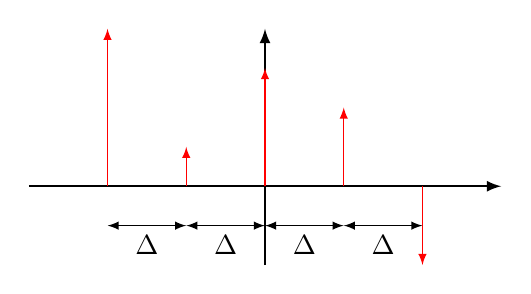
\begin{tikzpicture}
            \draw[thick,-latex] ( 0, -1) -- (0, 2);
            \draw[thick,-latex] (-3,  0) -- (3, 0);

            \draw[red,-latex] (-2,0) -- (-2, 2);
            \draw[red,-latex] (-1,0) -- (-1, 0.5);
            \draw[red,-latex] ( 0,0) -- ( 0, 1.5);
            \draw[red,-latex] ( 1,0) -- ( 1, 1);
            \draw[red,-latex] ( 2,0) -- ( 2,-1);

            \draw[latex-latex] (-2, -0.5) -- (-1, -0.5) node[midway, below] {$\Delta$};
            \draw[latex-latex] (-1, -0.5) -- ( 0, -0.5) node[midway, below] {$\Delta$};
            \draw[latex-latex] ( 0, -0.5) -- ( 1, -0.5) node[midway, below] {$\Delta$};
            \draw[latex-latex] ( 1, -0.5) -- ( 2, -0.5) node[midway, below] {$\Delta$};
        \end{tikzpicture}
        \caption{Uniform Interpolation}
    \end{subfigure}
    \hfil%
    \begin{subfigure}{0.45\linewidth}
        \centering
        \begin{tikzpicture}
            \draw[thick,-latex] ( 0, -1) -- (0, 2);
            \draw[thick,-latex] (-3,  0) -- (3, 0);

            \draw[red,-latex] (-2.5, 0) -- (-2.5,  2);
            \draw[red,-latex] (-0.5, 0) -- (-0.5,  0.5);
            \draw[red,-latex] ( 0  , 0) -- ( 0  ,  1.5);
            \draw[red,-latex] ( 1  , 0) -- ( 1  ,  1);
            \draw[red,-latex] ( 1.5, 0) -- ( 1.5, -1);
        \end{tikzpicture}
        \caption{Non-Uniform Interpolation}
    \end{subfigure}
\end{figure}

There are some important considerations when interpolating a function, but \textbf{shift-invariance} is the key point. If we shift the samples $\tilde{f}$ and apply the same interpolation, we should get a shifted version of the result $g$. 

Mathematically speaking, shifting the function would be equivalent to convolving with the impulse, \[ \tilde{f}(x, y) \ast \delta(x - \Delta_x, y - \Delta_y) = g(x, y) \ast \delta(x - \Delta_x, y - \Delta_y). \]

Consider a uniformly-sampled $f$ with period $\Delta$. 

\begin{figure}[ht!]
    \centering
    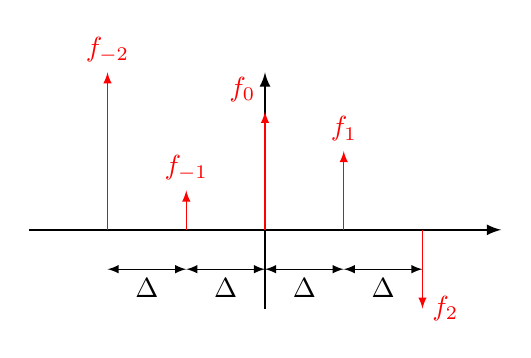
\begin{tikzpicture}
        \draw[thick,-latex] ( 0, -1) -- (0, 2);
        \draw[thick,-latex] (-3,  0) -- (3, 0);

        \draw[red,-latex] (-2,0) -- (-2, 2  ) node[above      ] {$f_{-2}$};
        \draw[red,-latex] (-1,0) -- (-1, 0.5) node[above      ] {$f_{-1}$};
        \draw[red,-latex] ( 0,0) -- ( 0, 1.5) node[above left ] {$f_0$};
        \draw[red,-latex] ( 1,0) -- ( 1, 1  ) node[above      ] {$f_1$};
        \draw[red,-latex] ( 2,0) -- ( 2,-1  ) node[      right] {$f_2$};

        \draw[latex-latex] (-2, -0.5) -- (-1, -0.5) node[midway, below] {$\Delta$};
        \draw[latex-latex] (-1, -0.5) -- ( 0, -0.5) node[midway, below] {$\Delta$};
        \draw[latex-latex] ( 0, -0.5) -- ( 1, -0.5) node[midway, below] {$\Delta$};
        \draw[latex-latex] ( 1, -0.5) -- ( 2, -0.5) node[midway, below] {$\Delta$};
    \end{tikzpicture}
\end{figure}

We observe that any interpolation methods that can be expressed as a linear shift-invariant transformation of the input samples must satisfy \[
    g(x) = \sum_{k=-\infty}^{\infty} f_k h(x - k\Delta),
\] where $h(x)$ is the interpolation filter (i.e. the interpolation kernel).

\begin{remark}
    $h(x - k\Delta)$ is $h(x)$ shifted by $k\Delta$. What we are saying here is that the final function $g$ will be a weighted sum of the shifted $h$ functions.
\end{remark}

In this course, we only consider \textit{uniform sampling} and \textit{LSI interpolations}.

\begin{example}
    Consider the interpolation filter $h$ 
    \begin{center} \begin{tikzpicture}
        \draw[thick,-latex] (-6, 0) -- (6, 0);
        \draw[thick,-latex] (0, -1) -- (0, 2);

        \draw[Light-Blue-600, thick, domain=-5.5:5.5, samples=100] plot (\x, {1/( (\x/3)^2 + 1 ) * cos((pi/2)*\x r)});
    \end{tikzpicture} \end{center}

    The $g$ function will be composed of many shifted copies of $h$.
    \begin{center} \begin{tikzpicture}
        \draw[thick,-latex] (-6, 0) -- (6, 0);
        \draw[thick,-latex] (0, -1) -- (0, 3);

        \draw[thick,red,-latex] (0, 0) -- (0, 2) node[above right] {$f_0$};

        \draw[Light-Blue-600, thick, domain=-5.5:5.5, samples=100] plot (\x, {2/( (\x / 3)^2 + 1 ) * cos((pi/2)*\x r)});
        \node[Light-Blue-600] at (2, 2) {$f_0 h(x)$};
    \end{tikzpicture} \end{center} \[
        g(x) = f_0 h(x) + \dots
    \] \begin{center} \begin{tikzpicture}
        \draw[thick,-latex] (-6, 0) -- (6, 0);
        \draw[thick,-latex] (0, -1) -- (0, 3);

        \draw[thick,red,-latex] (-2, 0) -- (-2,  2  ) node[above      ] {$f_{-2}$};
        \draw[thick,red,-latex] (-1, 0) -- (-1,  0.5) node[above      ] {$f_{-1}$};
        \draw[thick,red,-latex] ( 0, 0) -- ( 0,  1.5) node[above right] {$f_0$};
        \draw[thick,red,-latex] ( 1, 0) -- ( 1,  1  ) node[above      ] {$f_1$};
        \draw[thick,red,-latex] ( 2, 0) -- ( 2, -1  ) node[below      ] {$f_2$};

        \draw[Light-Blue-100, thick, domain=-4.5:0.5, samples=100] plot (\x, {2/( ((\x+2) / 3)^2 + 1 ) * cos(((pi/2)*(\x+2)) r)});
        \node[Light-Blue-100] at (-3, 2) {$f_{-1} h(x + 2\Delta)$};

        \draw[Light-Blue-400, thick, domain=-3.5:1.5, samples=100] plot (\x, {0.5/( ((\x+1) / 3)^2 + 1 ) * cos(((pi/2)*(\x+1)) r)});
        \node[Light-Blue-400] at (-2, 1) {$f_{-1} h(x + \Delta)$};

        \draw[Light-Blue-700, thick, domain=-2.5:2.5, samples=100] plot (\x, {1.5/( (\x / 3)^2 + 1 ) * cos(((pi/2)*\x) r)});
        \node[Light-Blue-700] at (2, 2) {$f_0 h(x)$};

        \draw[Light-Blue-A100, thick, domain=-1.5:3.5, samples=100] plot (\x, {1/( ((\x-1) / 3)^2 + 1 ) * cos(((pi/2)*(\x-1)) r)});
        \node[Light-Blue-A100] at (3, 1) {$f_1 h(x - \Delta)$};

        \draw[Light-Blue-A400, thick, domain=-0.5:4.5, samples=100] plot (\x, {-1/( ((\x-2) / 3)^2 + 1 ) * cos(((pi/2)*(\x-2)) r)});
        \node[Light-Blue-A400] at (4, -1) {$f_1 h(x - 2\Delta)$};

        % \addplot[red, mark=*] coordinates {(-2,2) (-1,0.5) (0,1.5) (0,0) (2,-1)};

        % Plot 7/60 x^5 + 1/6 x^4 - 11/12 x^3 - 11/12 x^2 + 0.105 x + 1.5
        \draw[ultra thick, Pink-700, domain=-2.25:2.5, samples=100] plot (\x, {(7/60) * (\x)^5 + (1/6) * (\x)^4 - (11/12) * (\x)^3 - (11/12) * (\x)^2 + 1.05 * (\x) + 1.5}) node[right] {$g(x)$};
    \end{tikzpicture} \end{center} \[
        g(x) = \cdots + f_{-1} h(x + 2\Delta) + f_{-1} h(x + \Delta) + f_0 h(x) + f_1 h(x - \Delta) + f_1 h(x - 2\Delta) + \cdots
    \]
\end{example}

\begin{itemize}
    \item Let $\tilde{f}$ be the function that defines the $k$ samples, \[
        \tilde{f} = \sum_{k=-\infty}^{\infty} f_k \delta(x - k\Delta).
    \] $f$ is non-zero only at the sample locations, and it is zero elsewhere.

    \item The interpolation process is LSI, so $g$ can be rxpressed as a convolution with some filter $h$, \[
        g = \tilde{f} \ast h = \left[ \sum_{k=-\infty}^{\infty} f_k \delta(x - k\Delta) \right] \ast h.
    \]

    \item Thus, we can express $g$ as \begin{align*}
        g & = \sum_{k=-\infty}^{\infty} f_k \left( \delta(x - k\Delta) \ast h \right) \\
          & = \sum_{k=-\infty}^{\infty} f_k h(x - k\Delta).
    \end{align*}
\end{itemize}

The interpolation filter is a \textbf{continuous function} over $x \in \mathbb{R}a$, but it \textbf{cannot be arbitrary}. To ensure $g(x)$ passes through all $f_k$, we need to ensure that $h(x)$ satisfies \begin{itemize}
    \item $h(0) = 1$ (interpolating the sample at $x = 0$)
    \item $h(k\Delta) = 0$ for all $k \neq 0$ (interpolating the sample at $x = k\Delta$)
\end{itemize} To ensure that $g(x)$ is smooth, we need \begin{itemize}
    \item $h(x)$ is smooth everywhere (i.e. continuous derivatives of all orders)
\end{itemize} Moreover, by having only few samples contributing to $g(x)$, efficiency can be ensured via local suppost: \begin{itemize}
    \item $h(x) = 0$ outside a small neighbourhood of $x = 0$
\end{itemize}

\subsection{Common Interpolation Filters}

\subsubsection{Nearest-Neighbour Interpolation}

% TODO: Complete this section

\subsubsection{Linear Interpolation}

% TODO: Add figure

\[
    g(x) = \left( 1 - \frac{x}{\Delta} \right) f_0 + \frac{x}{\Delta} f_1 \qquad \text{for } 0 \leq x < \Delta.
\]

% TODO: Derivation of the filter

\[
    h(x) = \begin{cases}
        1 - \frac{x}{\Delta} & 0 \leq |x| < \Delta, \\
        \frac{x}{\Delta}     & \text{otherwise}.
    \end{cases}
\]

% TODO: plot

It is easy to show that \[
    h(x) = \boxfn_{\Delta}(x) \ast \boxfn_{\Delta}(x) \cdot \frac{1}{\Delta}.
\]

\subsubsection{Bilinear Interpolation}

% TODO: figures

\[
    g(x, y) = \tilde{f}(x, y) \ast \left[ h(x) \cdot h(y) \right],
\], where $h(x)$ and $h(y)$ are the 1D linear interpolation kernels.

\subsubsection{Cubic Interpolation}

Form the stated desiderata it is possible to also derive a 3rd degree polynomial interpolation filter, \[
    h(x) = \begin{cases}
        \frac{3}{2} |s|^3 - \frac{5}{2} |s|^2 + 1 & 0 \le |s| < 1, \\
        -\frac{1}{2} |s|^3 + \frac{5}{2} |s|^2 - 4|s| + 2 & 1 \le |s| < 2, \\
        0 & \text{otherwise}.
    \end{cases} \qquad \text{where } s = \frac{x}{\Delta}.
\]

\begin{remark}[Why there are no second degree interpolation filters]
    Recall that we require the property that \begin{itemize}
        \item They have value $1$ at $0$, and 
        \item They go to $0$ at $\pm \Delta$ (i.e. the previous / next sample location).
    \end{itemize}

    It is impossible for a second degree polynomial to satisfy both of these properties.
\end{remark}

\section{Fourier Transform}

\subsection{The Fourier Transform}

Any periodic signal can be expressed as a sum of sines and cosines. The Fourier transform is a generalization of this idea to non-periodic signals.

In the \textbf{fourier domain}, a point in space no longer represents a value of the signal, but a \textit{frequency} of the signal.

\begin{figure}[ht!]
    \centering
    \begin{tikzpicture}
        \draw[thick,-latex] (-2, 0) -- (2, 0) node[right] {$\omega_x$};
        \draw[thick,-latex] (0, -2) -- (0, 2) node[right] {$\omega_y$};

        \fill[black] (0, 0) circle (0.1) node[below right] {$(0, 0)$};

        \node (x) at (3, -1) {Spacial frequency along $x$};
        
        \node (y) at (-3, 2) {Spacial frequency along $y$};
    \end{tikzpicture}

    \caption{The Fourier domain of a constant-intensity image (the ``DC component'')}
\end{figure}

\begin{example}
    The points in the Fourier domain represent the frequencies of the signal.

    \begin{itemize}
        \item The point $(5, 0)$ represents an image that varies sinusoidally along $x$ with a frequency of $5$ cycles per unit length. 
        \item The point $(0, 5)$ represents an image that varies sinusoidally along $y$ with a frequency of $5$ cycles per unit length.
    \end{itemize}

    The larger the magnitude of the point, the higher the frequency of the sinusoid.

    \begin{figure}[ht!]
        \centering
        \includegraphics[width=0.25\linewidth]{figures/stp1fil1.png}

        \caption{The image in the spatial domain corresponds to point $(17, 17)$ in the Fourier domain.}
    \end{figure}
\end{example}

Merely specifying the frequencies $(\omega_x, \omega_y)$ is \textbf{not} sufficient to uniquely determine the image. We need the sinusoid to have a \textit{phase} as well. The general expression for the intensity of pixel $(x, y)$ represented by $(\omega_x, 0) \& (-\omega_x, 0)$ is given by \[
    I(x, y) = \cos \left( \omega_x \frac{2\pi}{C} x + \varphi \right),
\] and similarly, the general expression for the intensity of pixel $(x, y)$ represented by $(0, \omega_y) \& (0, -\omega_y)$ is given by \[
    I(x, y) = \cos \left( \omega_y \frac{2\pi}{R} y + \varphi \right).
\] Thus, the general expression for image represented by $(\omega_x, \omega_y)$ is given by \[
    I(x, y) = \cos \left[ \left( \omega_x \frac{2\pi}{C} x \right) + \omega_y \left( \frac{2\pi}{R} y + \varphi \right) \right].
\]

To properly account for phase, $(\omega_x, \omega_y)$ actualy represents an image whose intensities are \textit{complex-valued}. The image will have a real component and an imaginary component, and the phase of the sinusoid is given by the angle of the complex number, \[
    I(x, y) = \cos(2\pi \frac{x}{C} \omega + \varphi) + j \sin(2\pi \frac{x}{C} \omega + \varphi).
\]